\section{Introduction}

\todo{Is halt die frage ob ma den anfang einfach so schreiben, war ja eigentlich net ganz so xD}

Mobile apps are utilized for virtually all aspects of daily life in the modern world. So after we noticed that there is no application that allows the efficient planning of campaigns like the "Sternsinger-Aktion" we asked ourselves why, and furthermore, how hard it is to create an App with intuitive usability with the main purpose of simplifying the process of managing such a campaign and gaining a general overview of the progress made by the groups.

\blankLine

The app needs to comply with specific criteria we defined in cooperation with Prof. DI Robert Müllerferli. He is the main organizer of the campaign in the parish of Lieboch and helped us to work out the key aspects our project should implement. In the finished product, every user should be able to scan a QR-Code, through which the area of this group gets assigned to the device. These areas must be dynamically adjustable, so an admin can coordinate the workload of each area more efficiently. The areas also need to be clearly visible by an outline which gets drawn through "Border" addresses. These border addresses get calculated by an algorithm implemented by us. It should be visible at a glance if there is an "specification", which can be assigned by admins, set for an address. This should be realized through the use of different icons instead of the default icon. Apart from the app itself, we also implemented a web-portal through which administrators can manage and supervise the campaign. 

\todo{vielleicht noch was rein bezüglich der borders und dann unten nurmehr drauf referenzieren?}

\blankLine

The research part of this thesis will be dedicated to how components should act and look, so that new users can use this tool without requiring a long "onboarding" phase. It should feel familiar to interact with elements and the borders of what users can and can not do need to be clearly defined. Because our application also needs a reliable data source to guarantee the consistency and accuracy of marked addresses, we researched ways to keep our database up-to-date, without the need of much manual intervention. After defining the project requirements, we noticed that we need to calculate which addresses are border addresses. So we decided to take a look into different algorithms for this task and compare them concerning their efficiency, decide on one of them and implement it.

\blankLine

This thesis contains an in-depth description of our thought and development
process, as well as any other steps we took to achieve our goal of a
functional mobile application that can be used by volunteers in course of the
"Sternsinger-Aktion 2025" taking place in the parish of Lieboch.

\newpage

\subsection{Team}


This thesis was created by three Students attending the BHIF20 at the
HTBLA Kaindorf Computer Science Department.

\blankLine

\todo{andis bild anpassen}

\begin{center}
    \begin{tabularx}{\textwidth}{X X X}
        \centering
        \textbf{\daAuthorOne} \newline
        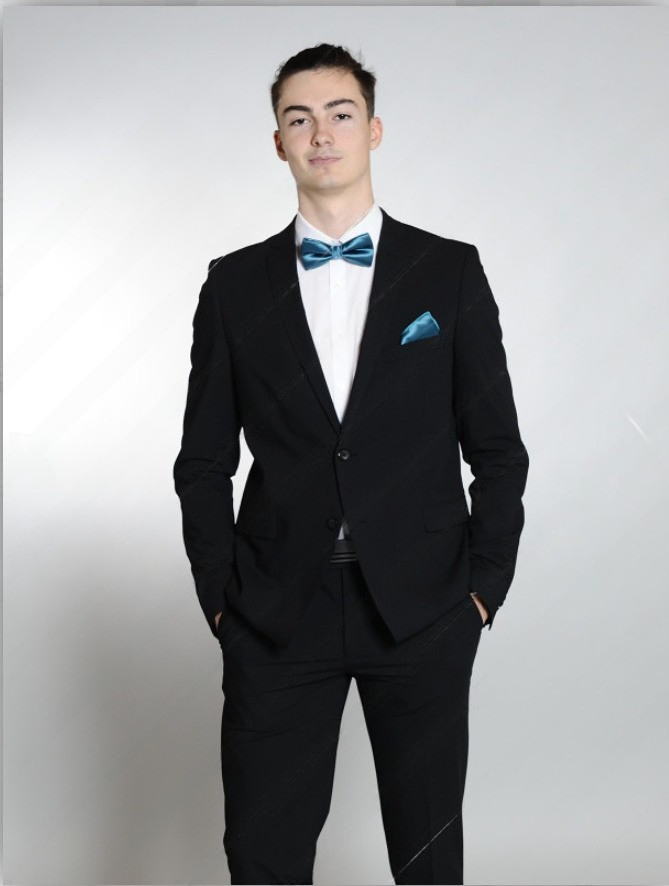
\includegraphics[width=0.28\textwidth]{images/people/leonEdlinger.jpeg} \newline
        Database, Admin-Panel &
        
        \centering
        \textbf{\daAuthorTwo} \newline
        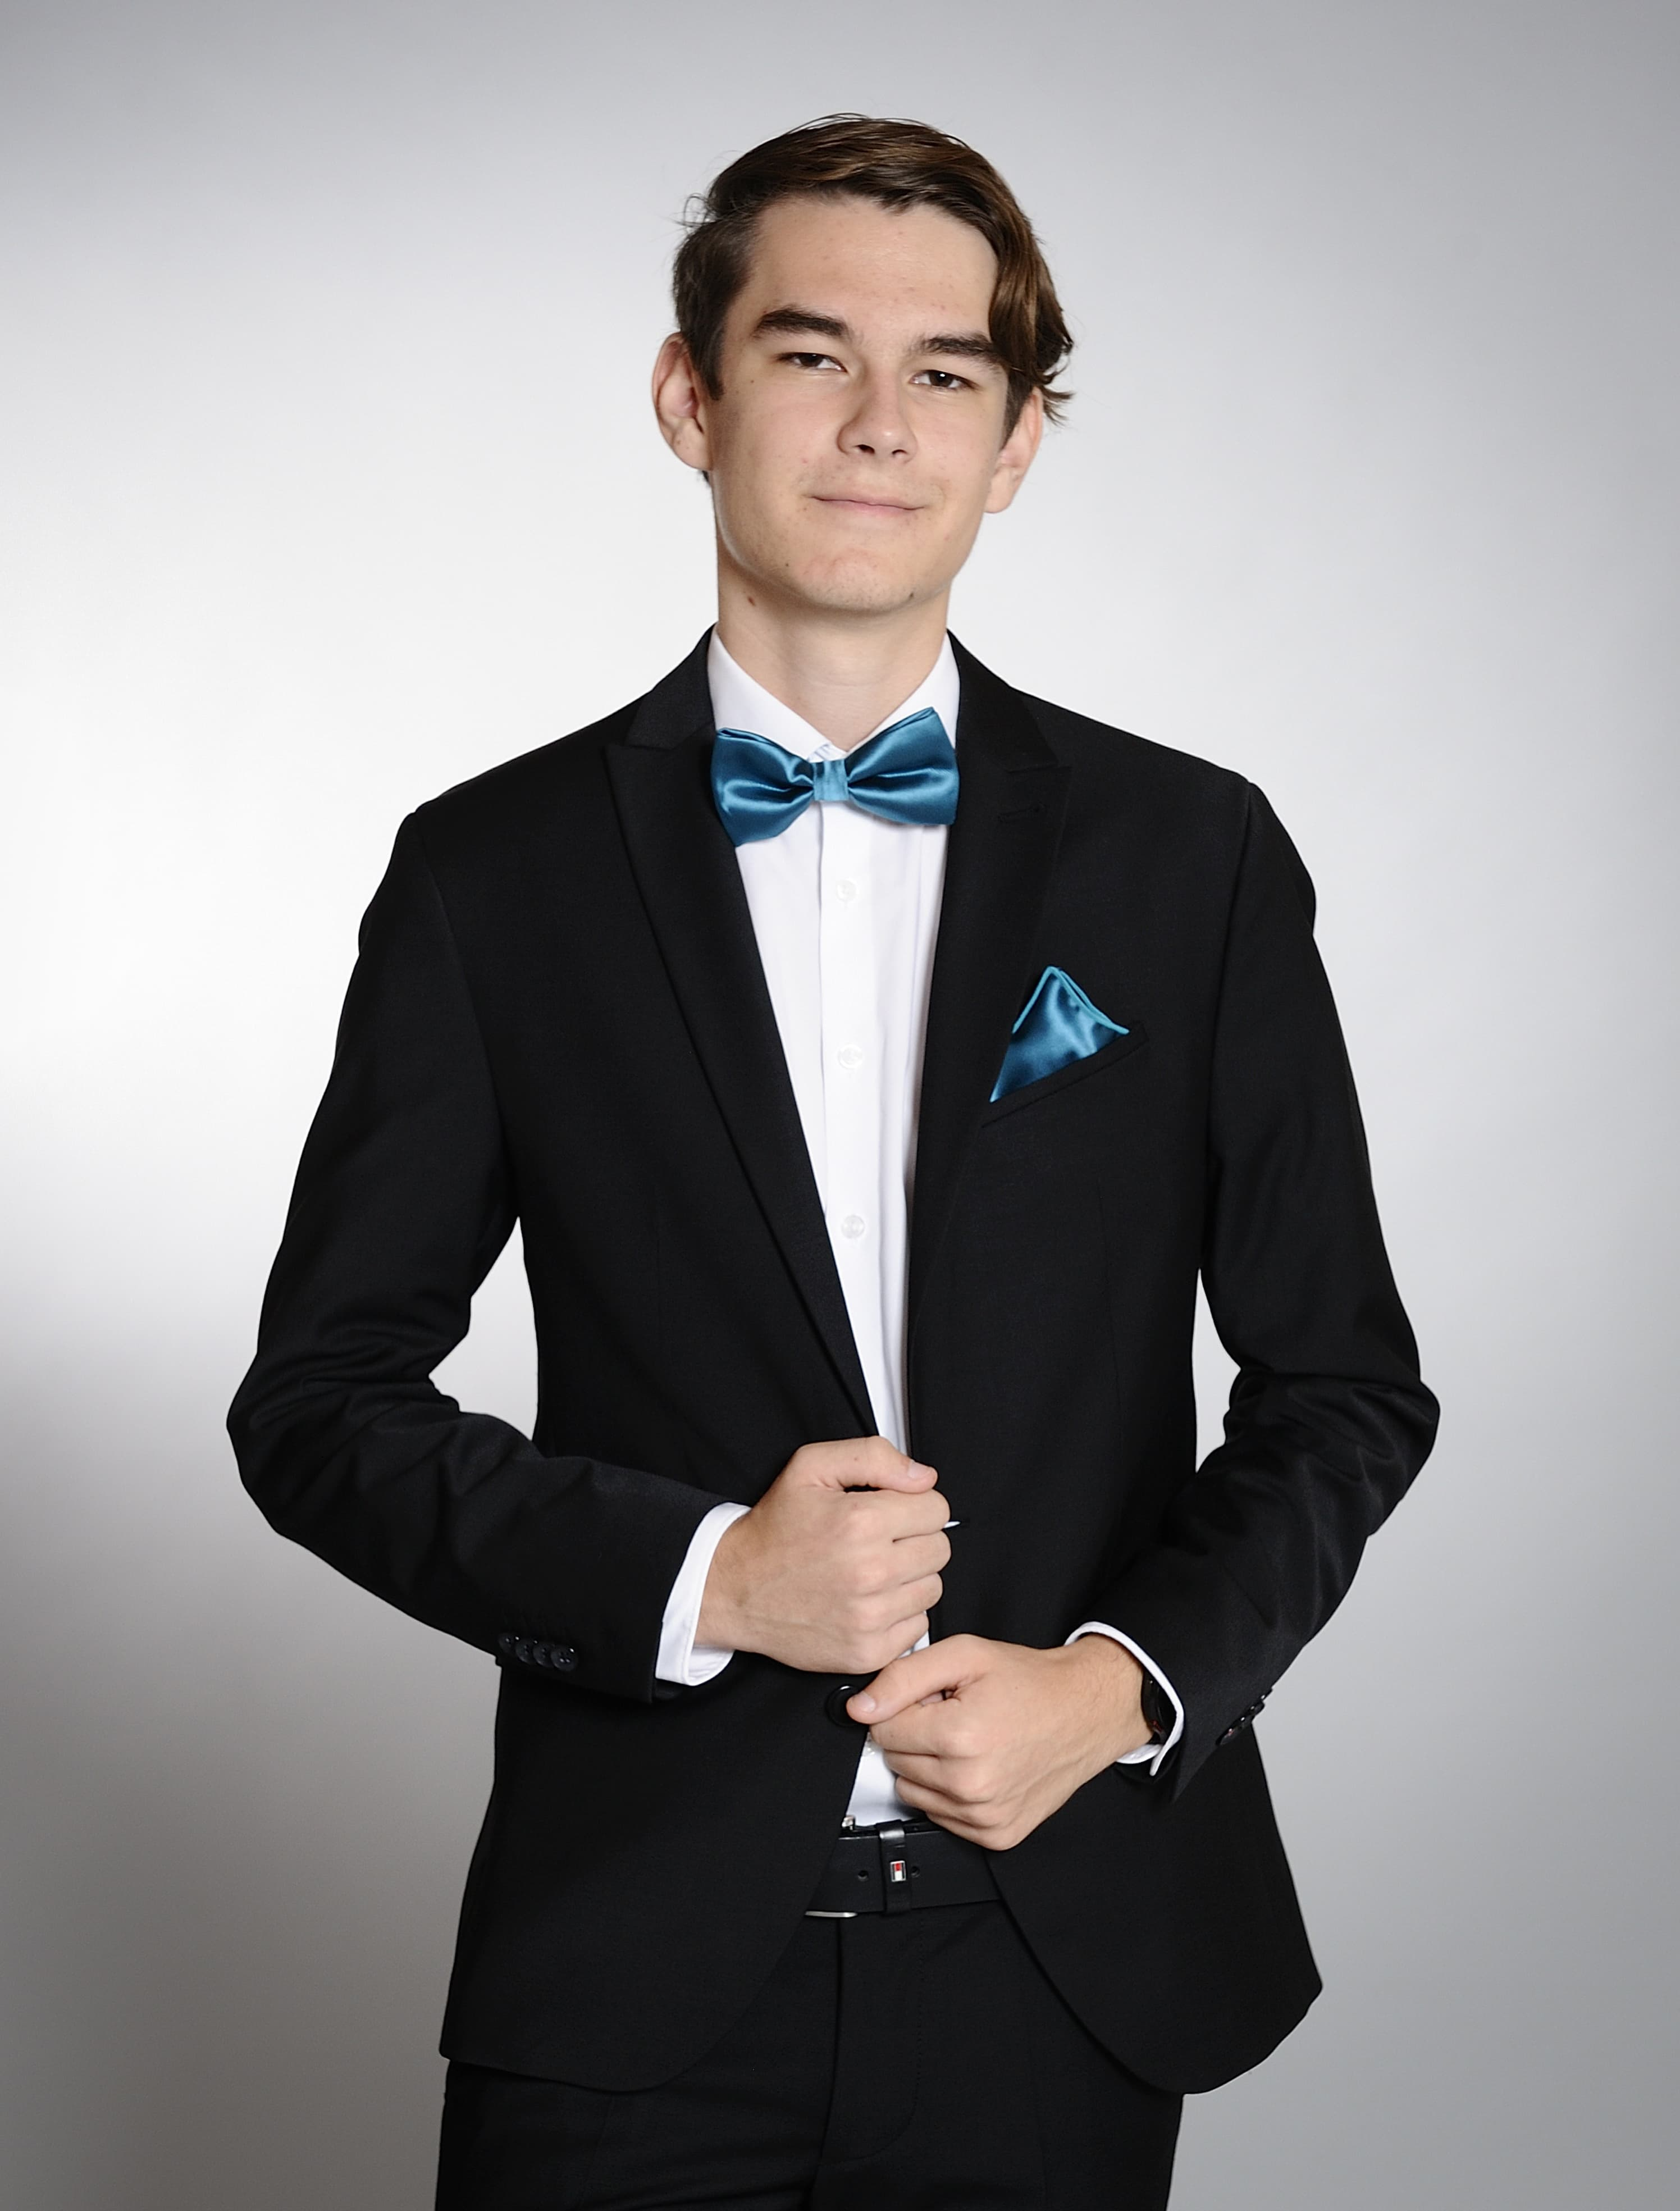
\includegraphics[width=0.28\textwidth]{images/people/paulGigler.jpeg} \newline
        Deployment, Mobile App &
    
        \centering
        \textbf{\daAuthorThree} \newline
        
\includegraphics[width=0.28\textwidth]{images/people/andreasWeissl.jpeg} \newline
        Backend
    \end{tabularx}
    \end{center}

\newpage